%!TEX root = ../../anforderungsspezifikation.tex
\chapter{Funktionale Anforderungen / Use Case}

	\section{Use Case Diagramm}    
    \begin{figure}[h]
    	\centering
    	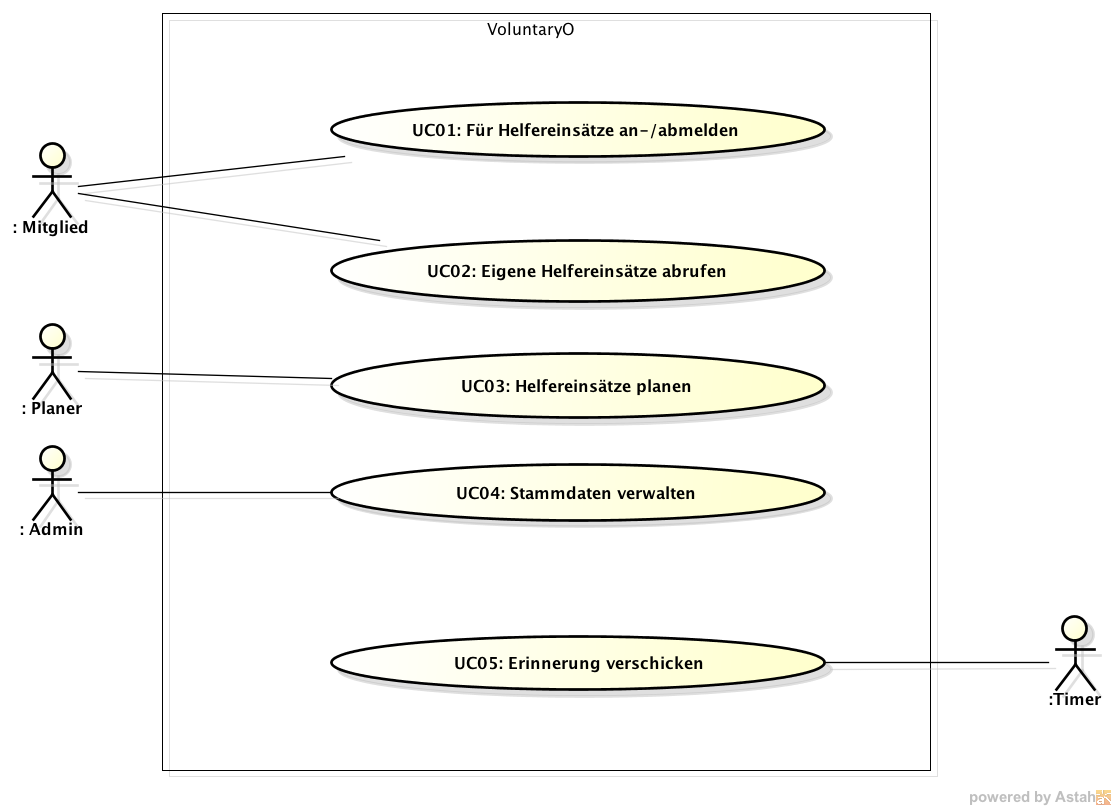
\includegraphics[width=0.9\textwidth]{content/anforderungsspezifikation/images/usecase_diagram.png}
    	\caption{Use Case Diagramm}
	\end{figure}
	
	\section{Use Cases brief Format}
    
    \begin{table}[H]
        \tablestyle
        \tablealtcolored
        \begin{tabularx}{\textwidth}{l X l}
            \tablebody
            \textbf{Use Case Name} &
                UC01: Für Helfereinsatz an-/abmelden
                \tabularnewline
            \textbf{Ref. Primäre Funktionen} &
                \textit{F08}, \textit{F09}
                \tabularnewline
            \textbf{Zusammenfassung} &
                Für jedes Event gibt es vorgegeben Helfereinsätze ( = „Tätigkeiten“). Benutzer können sich für diese Tätigkeiten eintragen und auch wieder abmelden.
                \tabularnewline
            \textbf{Main Success Szenario} &
                Benutzer wählt Helfereinsatz aus und meldet sich dafür an oder ab. System überprüft Fähigkeiten des Mitglieds und Sperrfrist und lässt An- bzw. Abmeldung zu, falls Sperrfrist nicht überschritten wurde.
                \tabularnewline
                \textbf{Actors} &
                User
                \tabularnewline
                \textbf{Extends} &
                
                \tabularnewline
            \tableend
        \end{tabularx}
    \end{table}
    
    \begin{table}[H]
        \tablestyle
        \tablealtcolored
        \begin{tabularx}{\textwidth}{l X l}
            \tablebody
            \textbf{Use Case Name} &
                UC02: Eigene Helfereinsätze anzeigen 
                \tabularnewline
            \textbf{Ref. Primäre Funktionen} &
                \textit{F10}
                \tabularnewline
            \textbf{Zusammenfassung} &
                Benutzer kann sich seine Helfereinsätze anzeigen lassen.
                \tabularnewline
            \textbf{Main Success Szenario} &
                Benutzer fragt Helfereinsätze ab. System liefert alle Helfereinsätze, für die der Benutzer angemeldet ist.
                \tabularnewline
                \textbf{Actors} &
                User
                \tabularnewline
                \textbf{Extends} &
                
                \tabularnewline
            \tableend
        \end{tabularx}
    \end{table}
    
    \begin{table}[H]
        \tablestyle
        \tablealtcolored
        \begin{tabularx}{\textwidth}{l X l}
            \tablebody
            \textbf{Use Case Name} &
                UC03: Helfereinsätze planen
                \tabularnewline
            \textbf{Ref. Primäre Funktionen} &
                \textit{F01}, \textit{F02}
                \tabularnewline
            \textbf{Zusammenfassung} &
                Jeder Event hat mehrere Helfereinsätze. Diese müssen vom Planer verwaltet werden.
                \tabularnewline
            \textbf{Main Success Szenario} &
                Der Planer kann verschiedene Helfereinsätze hinzufügen und diese ändern.
                \tabularnewline
                \textbf{Actors} &
                Planer
                \tabularnewline
                \textbf{Extends} &
                
                \tabularnewline
            \tableend
        \end{tabularx}
    \end{table}
    
    \begin{table}[H]
        \tablestyle
        \tablealtcolored
        \begin{tabularx}{\textwidth}{l X l}
            \tablebody
            \textbf{Use Case Name} &
                UC04: Stammdaten verwalten
                \tabularnewline
            \textbf{Ref. Primäre Funktionen} &
                \textit{F06}
                \tabularnewline
            \textbf{Zusammenfassung} &
                Die verschiedenen Benutzer sollen vom Admin verwaltet werden. Neue Benutzer sollen hinzugefügt werden können oder Passwörter geändert werden.
                \tabularnewline
            \textbf{Main Success Szenario} &
                Der Admin kann einen neuen Benutzer hinzufügen und dessen Passwort und Rolle setzen.
                \tabularnewline
                \textbf{Actors} &
                Admin
                \tabularnewline
                \textbf{Extends} &
                
                \tabularnewline
            \tableend
        \end{tabularx}
    \end{table}
    
    \begin{table}[H]
        \tablestyle
        \tablealtcolored
        \begin{tabularx}{\textwidth}{l X l}
            \tablebody
            \textbf{Use Case Name} &
                UC05: Erinnerung verschicken
                \tabularnewline
            \textbf{Ref. Primäre Funktionen} &
                \textit{F11}
                \tabularnewline
            \textbf{Zusammenfassung} &
                Für jeden Event sollen an vordefinierten Zeitpunkten Erinnerungen an alle angemeldeten Benutzer versendet werden können.
                \tabularnewline
            \textbf{Main Success Szenario} &
                Es wird automatisch eine Erinnerung an jeden im Event angemeldeten Benutzer gesendet.
                \tabularnewline
                \textbf{Actors} &
                Timer
                \tabularnewline
                \textbf{Extends} &
               	
                \tabularnewline
            \tableend
        \end{tabularx}
    \end{table}
